\documentclass{standalone}
\begin{document}
	\subsection{Visual Comparison}
	
	In this subsection I will discuss the segmentation results. The segmentation obtained by the pipeline were compared with the manual segmentation provides within the dataset. This comparison aims to match the different modality for patient that presents a regular lesion pattern. 
	
	\begin{figure}[h!]
		\centering
			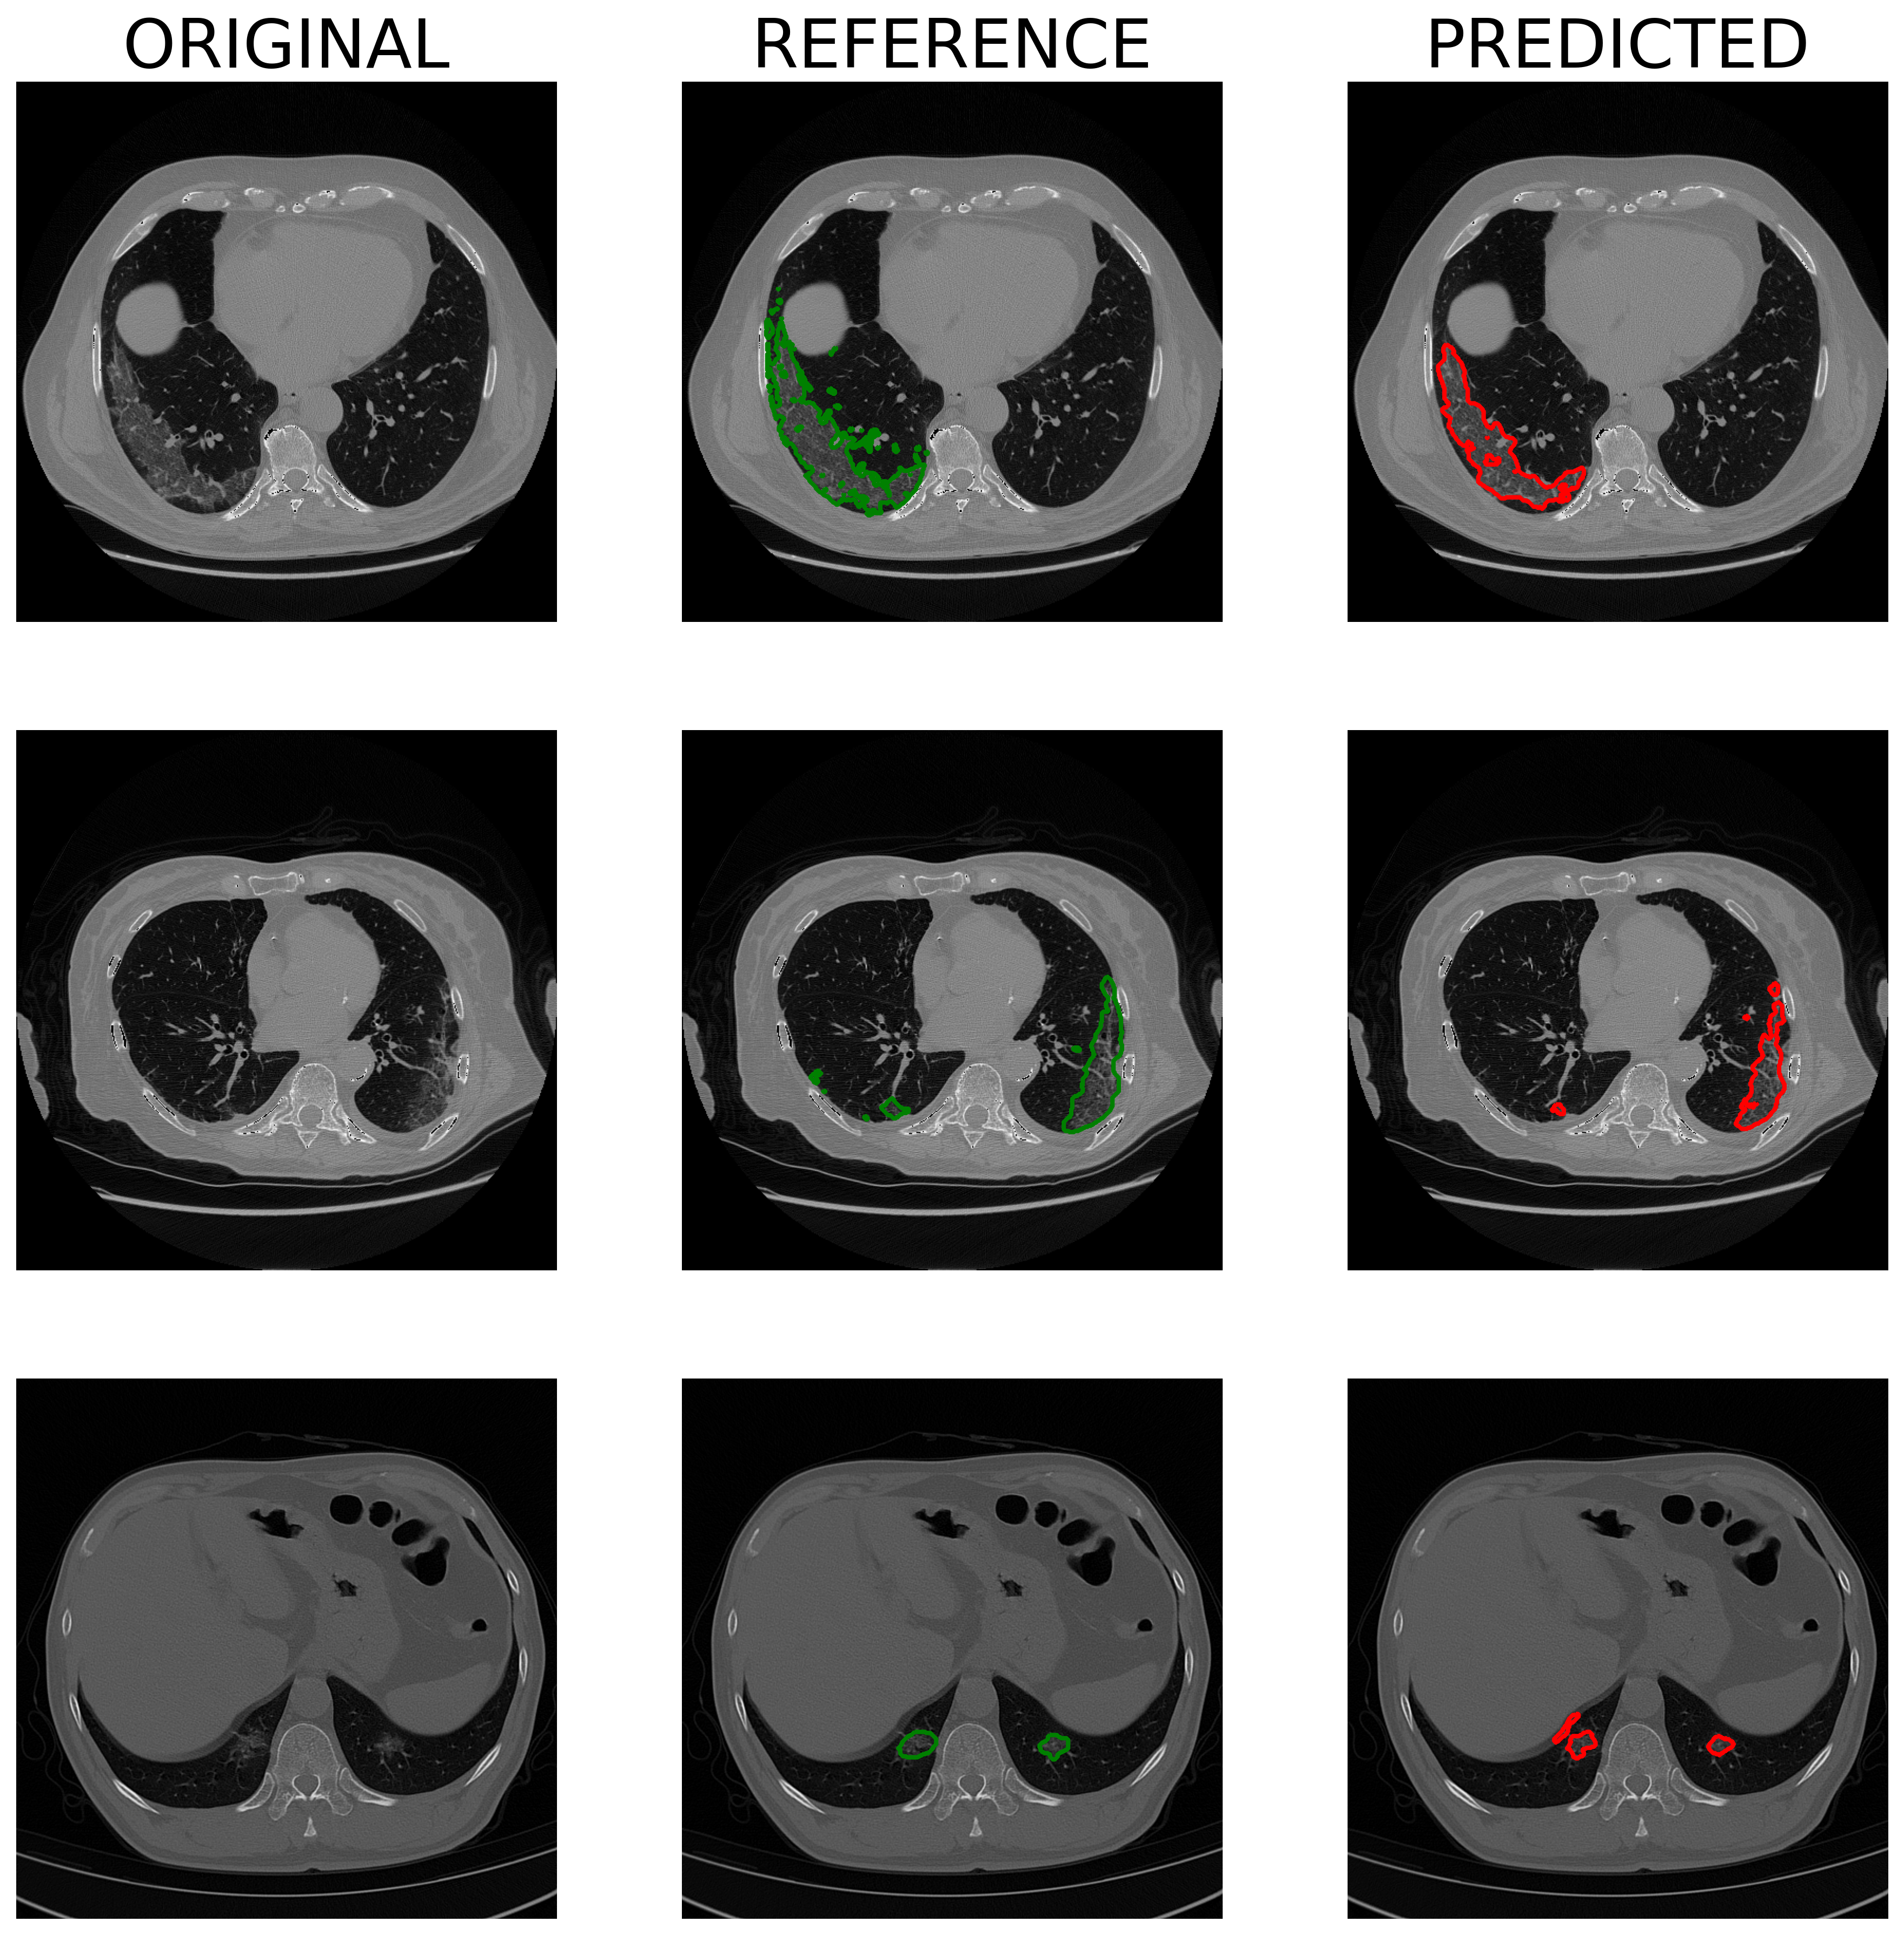
\includegraphics[scale=.4]{Results1.png}
			\caption{Comparison between the lesion areas detected by the developed pipeline(red) and te reference ones(green). We can see how the the lesion areas are correctly detected. }\label{fig:Results}
	\end{figure}

	In \figurename\,\ref{fig:Results} I've reported a comparison between the segmentation achieved by the developed pipeline(red) and the reference labels(green) for three scans of patient with a typical lesion pattern. We can see how the lesion areas are correctly identified. We can observe how in each case the edges of the label estimated by the pipeline are more detailed respect to the reference ones; and the first case the achieved segmentation presents less false positives.\\ In the last scan we can observe how in presence of motion artifacts the pipeline may presents false positives; but the lesion areas are well segmented.
	
	
\end{document}